\section{Geometría Riemanniana}
\begin{frame}
	\frametitle{Variedades Riemannianas}
	\begin{definition}[Métrica Riemanniana]
		Sea $M$ una variedad suave. Una \bf{Métrica Riemanniana} $g$ en $M$ es un campo suave 2-tensorial covariante simétrico, el cual es definido positivo en cada punto.
	\end{definition}
\end{frame}

\begin{frame}
	\frametitle{Variedades Riemannianas}
	\begin{columns}
		\column{0.4\textwidth}
		\begin{enumerate}
			\item<1-> Campo suave
			\item<2-> $2-$tensor covariante
			\item<3-> Simétrico.
			\item<4-> Definido positivo.
		\end{enumerate}
		\column{0.6\textwidth}
		\only<1>{
			\begin{figure}[t]
				\includegraphics[scale=0.25]{Figuras/CampoVectorial.png}
				\caption{Campo vectorial suave}
			\end{figure}
		}

		\only<2>{ \begin{align*}
				g_p(-,-)               : & T_{p}M \times T_{p}M \to \mathbb{R} \\[10pt]
				g_p(\lambda x + y, z)    & = \lambda g_p(x,z) + g_p(y,z)       \\
				g_p(x,\lambda y + z)     & = \lambda g_p(x,y) + g_p(x,z)       \\
			\end{align*} }
		\only<3>{\[
				g_p(x,y) = g_p(y,x)
			\]}
		\only<4>{\begin{align*}
				g_{p}(x,x) & > 0, \quad \text{ si } x \neq 0 \\
				g_{p}(0,0) & = 0, \quad \text{ si } x = 0
			\end{align*} }

		\only<5> {
			\begin{figure}[t]
				\scalebox{0.75}{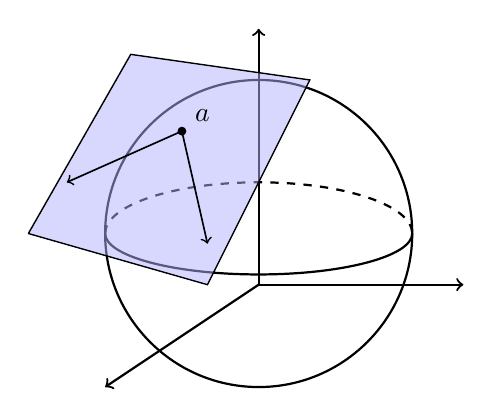
\begin{tikzpicture}[scale=0.65]
	% Esfera
	\draw [thick] (3,0) arc (0:180:3 and -0.8);
	\draw [thick, dashed] (-3,0) arc (180:0:3 and 1);
	\draw [thick] (0,0) circle (3);

	% Ejes R3
	\draw [thick,->] (0,-1) -- (0,4);
	\draw [thick,->] (0,-1) -- (4,-1);
	\draw [thick,->] (0,-1) -- (-3,-3);


	% Rectángulo (Espacio Tangente)
	\draw [fill=blue!30!white,opacity=0.5, line width=0] (-4.5,0) -- (-2.5,3.5) --(1,3.0) -- (-1,-1) -- (-4.5,0);
	\draw [line width=0.5] (-4.5,0) -- (-2.5,3.5) --(1,3.0) -- (-1,-1) -- (-4.5,0);
	\filldraw (-1.5,2) circle (0.075);
	\node at (-1.1,2.3) {$a$};


	\draw [semithick, ->] (-1.5,2) -- (-1,-0.2);
	\draw [semithick, ->] (-1.5,2) -- (-3.75,1);
\end{tikzpicture}
}
			\end{figure}
		}
	\end{columns}

	\vspace{24pt}

	\only<5>{ En pocas palabras, una métrica Riemanniana define un producto interno en el espacio tangente a cada punto de una variedad suave.}
	\only<6> {\begin{definition}[Variedad Riemanniana]
			El par $(M,g)$, donde $M$ es una variedad suave y $g$ es una métrica Riemanniana, es llamado un \textbf{Variedad Riemanniana}. \end{definition} }
\end{frame}

\begin{frame}
	\frametitle{Variedades Riemannianas}
	\begin{lemma}[Expresión local de la métrica]
		\label{Lemma: Expresión local de la métrica}
		Sean $(M,g)$ una variedad Riemanniana, $p \in M$ y $(U,\phi)$ una carta suave que contiene a $p$. La métrica puede expresarse de manera local en $U$ como:
		\[
			g = \sum_{i=1}^{n}\sum_{j=1}^{n} g_{ij} d\phi_i d\phi_j,
		\]
		donde $\{ d\phi_{1}, \ldots, d\phi_{n} \}$ es la base del espacio dual a $T_{p}M$, asociada a la base $\{ \partial \phi_{1}, \ldots, \partial \phi_{n} \}$, y $g_{ij}$ son funciones suaves dadas por:
		\[
			g_{ij}(p) = g_{p}\left( \partial \phi_{i} \big|_{p}, \partial \phi_j \big|_{p}\right)
		\]
	\end{lemma}
\end{frame}

\begin{frame}
	\frametitle{Variedades Riemannianas}
	Dada una métrica $g$ es posible asociar a esta una matriz $G$, la cual depende de las coordenadas locales de la carta sobre la cual esté definida. \pause Las entradas de $G$ son las funciones $g_{ij}$ definidas anteriormente.
	\[
		G = \begin{bmatrix}
			g_{11} & g_{12} & \cdots & g_{1n} \\
			g_{21} & g_{22} & \cdots & g_{2n} \\
			\vdots & \vdots & \ddots & \vdots \\
			g_{n1} & g_{n2} & \cdots & g_{nn}
		\end{bmatrix}
	\]\pause

	\vspace{12pt}

	La matriz $G$ es simétrica y definida positiva.
\end{frame}


\begin{frame}
	\frametitle{Métrica Euclidiana}\pause
	\begin{example}
		En $\mathbb{R}^{n}$ con la base estándar $\{x_{1}, \ldots, x_{n}\}$ definimos la métrica:
		\[
			g = \sum_{i=1}^{n} \sum_{j=1}^{n} \delta_{ij} dx_{i} dx_{j} = \sum_{i=1}^{n} \left(dx_{i}\right)^{2}
			\only<3>{, \quad G = I_{n \times n}}
		\] \pause \pause
		Aplicando esta métrica a dos vectores tangentes arbitrarios $v = \begin{bmatrix} v_1 \cdots v_n \end{bmatrix}$ y $w = \begin{bmatrix} w_1 \cdots w_n \end{bmatrix}$ se obtiene:
		\begin{align*}
			g(v,w) & = \sum_{i=1}^{n} dx_{i}(v) dx_{i}(w)   \\
			       & = \sum_{i=1}^{n}v_{i}w_{i} = v \cdot w
		\end{align*}
	\end{example}
\end{frame}

\begin{frame}
	\frametitle{Variedades Riemannianas}\pause
	\begin{theorem}[Existencia de la métrica] Toda variedad suave puede ser equipada con una métrica Riemanniana.
	\end{theorem}\pause
	\begin{proof}
		\begin{enumerate}
			\item Sea $M$ una variedad suave y $(U_{\alpha},\phi_{\alpha})$ cualquier carta suave en $M$. \pause
			\item Dado un punto $p$ en la carta $(U_\alpha,\phi_\alpha)$ y dos vectores tangentes $v,w$ en $T_{p}M$ como, podemos expresar a estos como una combinación lineal:
			      \[
				      v = \sum_{i=1}^{n} v_{i} \partial \phi_{i}, \quad
				      w = \sum_{j=1}^{n} w_{j} \partial \phi_{j},
			      \]
		\end{enumerate}
	\end{proof}
\end{frame}

\begin{frame}
	\begin{proof}
		\begin{enumerate}
			\setcounter{enumi}{2}
			\item Definimos en $U_{\alpha}$ la métrica $g^{\alpha}$ como:
			      \[
				      g_{p}^{\alpha}(v,w) = \sum_{i=1}^{n}\sum_{j=1}^{n} \delta_{ij} v_{i}w_{j} = \sum_{i=1}^{n} v_{i} w_{i}
			      \] \pause
			\item Utilizando una partición de la unidad $\{f_{\alpha}\}$ subordinada a la estructura suave de $M$ se construye una métrica global $g$, de tal modo que:
			      \[
				      g_p = \sum_{\alpha} f_{\alpha} g_{p}^{\alpha}
			      \]
		\end{enumerate}
	\end{proof}
\end{frame}

\begin{frame}
	\begin{figure}[t]
		\scalebox{0.75}{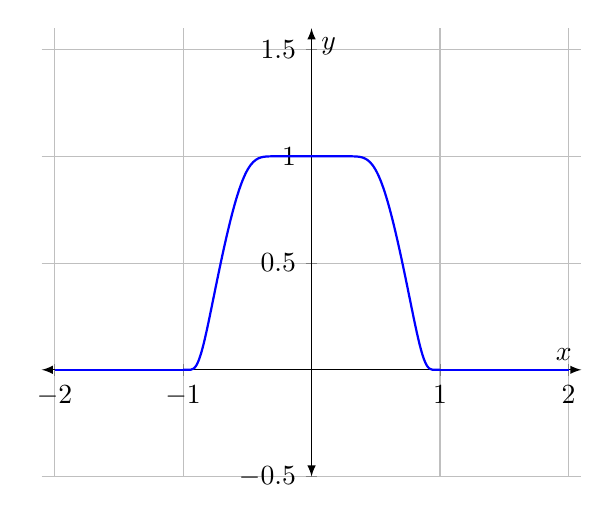
\begin{tikzpicture}
\begin{axis}[
  grid=both,
  xmin=-2.1,
  xmax=2.1,
  ymin=-0.5,
  ymax=1.6,
  axis lines=middle,
  xlabel = $x$,
  ylabel = $y$,
  axis line style={latex-latex},
  ]

\addplot[
  samples=100,
  domain=-1:1,
  color=blue,
  thick,
  smooth,
  ]
  {1 -( ((e)^(-1/(x^2))) / ( ( e^(-1/(x^2)) ) + (e^(-1/(1-(x^2)))) ))};


\addplot[
  samples=2,
  domain=-2:-0.99,
  color=blue,
  thick,
  smooth
  ]
  {0};

\addplot[
  samples=2,
  domain=0.99:2,
  color=blue,
  thick,
  smooth
  ]
  {0};
\end{axis}
\end{tikzpicture}
}
		\caption{Gráfica de una función indicadora suave.}
	\end{figure}
\end{frame}
